\chapter{TTL and multiplexer}
In this session we first measured the latency between the input and output signal of a 74LS00, then we used a NOT gate with open collector to turn on and off a LED, thirdly we designed and built an half dulpex with two 3state gates and lastly we designed and implemented a multiplexer with 4 signals and two bit of selection.

\section{Materials}
\begin{itemize}
\item A resistor
\item A LED
\item Power supply RIGOL DP831A
\item Waveform generator RIGOL DG1032
\item Multimeter RIGOL DM3068
\item 74LS00
\item 74LS05
\item 74LS04
\item 74LS125
\end{itemize}

\section{Experimental setup}
For measuring the time propagation of the signal in the 7400 we used the configuration in figure \ref{latency}. As input we used a square wave with 0-5 V voltage and the frequency of 100kHz.
\begin{figure}[H]
\centering
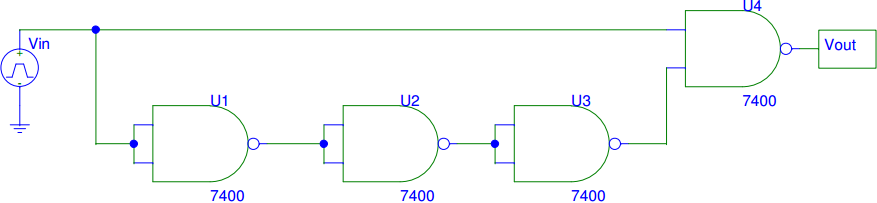
\includegraphics[width=.7\textwidth]{10/latency.png}
\caption{The circuit used for measuring the latency in the propagation of a digital input}\label{latency}
\end{figure}
For testing the NOT gate we implemented a circuit for switching on and off the LED. The circuit is in figure \ref{LED_ON_OFF} with a power supply of 9 V and a pull-up resistor of 1 k$\Omega$.
\begin{figure}[H]
\centering
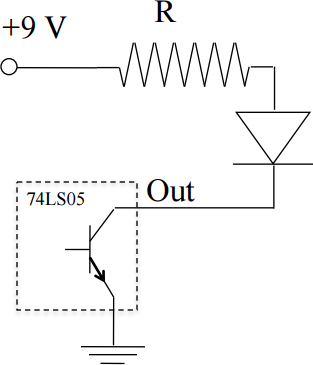
\includegraphics[width=.3\textwidth]{10/LED_ON_OFF.png}
\caption{NOT TTL Open Collector}\label{LED_ON_OFF}
\end{figure}
For the half duplex we built it as in figure \ref{TTL_3state}, we connected the two input by first passing the signals (a square wave and the other was connected to ground) into a 3state that had the enable bits opposite to one another, so just one signal passed at the time. It was possible to change signal by changing the voltage (0-5 V) in S.
\begin{figure}[H]
\centering
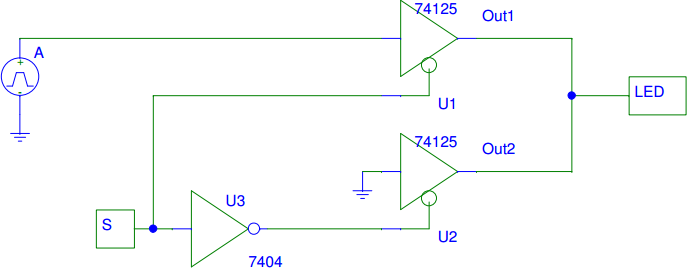
\includegraphics[width=.7\textwidth]{10/TTL_3state.png}
\caption{Half duplex used for sharing a transmission channel}\label{TTL_3state}
\end{figure}

Lastly we designed a mutiplexer to pass 4 different signals to another group. First we needed to design a selector to choose between the 4 signals with 2 bits, this was implemented with the circuit \ref{multi_select}.
\begin{figure}[H]
\centering
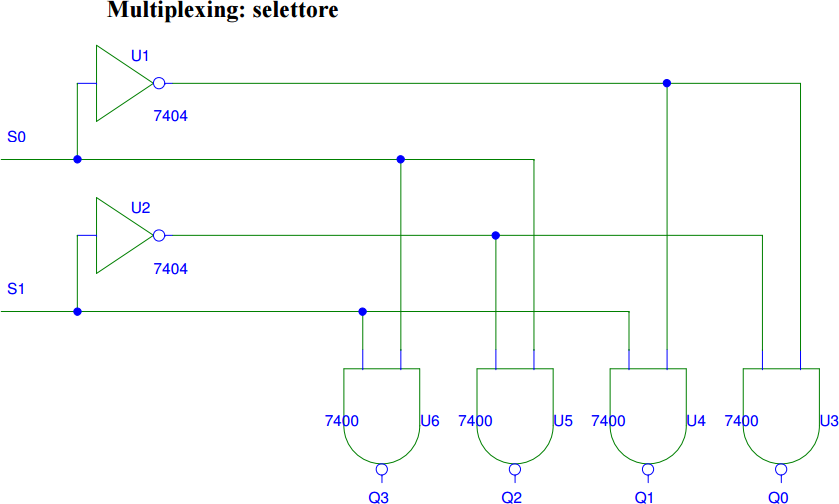
\includegraphics[width=.7\textwidth]{10/multi_select.png}
\caption{The selection circuit, the choice of the enabled channel is made with the 2 bits S0,S1}\label{multi_select}
\end{figure}
Then we used the signals from the selector to enable and disable 4 3state gates that were connected with channels D0,D1,D2,D3, this was done in a similar way to the half duplex as we can see the circuit in \ref{multi_wired}.
\begin{figure}[H]
\centering
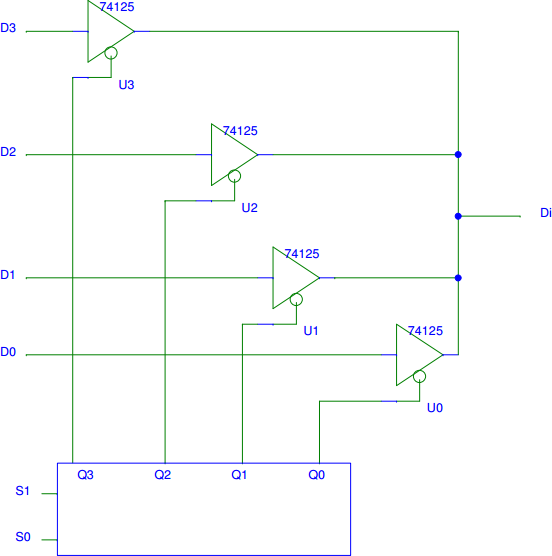
\includegraphics[width=.7\textwidth]{10/multi_wired.png}
\caption{The signal from the multiplexer used for blocking and allowing the chosen channel}\label{multi_wired}
\end{figure}
\begin{table}[H]
\centering
\begin{tabular}{c|c|c}
 S0 & S1 & Channel enabled\\
 \hline
 0 & 0   & D0\\
 0 &1    &  D1\\
 1&0    & D2\\ 
 1 &1    &  D3\\ 
\end{tabular}\caption{The circuit works with this table of selection}

\end{table}

Then we took the signal from the output of the 3state gates Di and passed to our friends with a cable, we also transmitted the two bits of selection, for allowing them to know which channel was transmitting. The common reference used by the 2 group was the common ground of the building, we successfully trasmitted various signal to the other side of the room 

\section{Data analysis}
In the plot \ref{latency_plot} we can evaluate the time delay caused by the single gate. We see that the signal from the point it started descending to the point it started going up, it took about 14 ns, that divided by the three gates gives about 4.7 ns per gate. We chose the starting point when the output has a negative derivative, because that is the moment when the first pin receives the signal, and we chose the ending time when the signal invertes direction, because that is the moment when the second signal is propagated in all the three gates.
\begin{figure}[H]
\centering
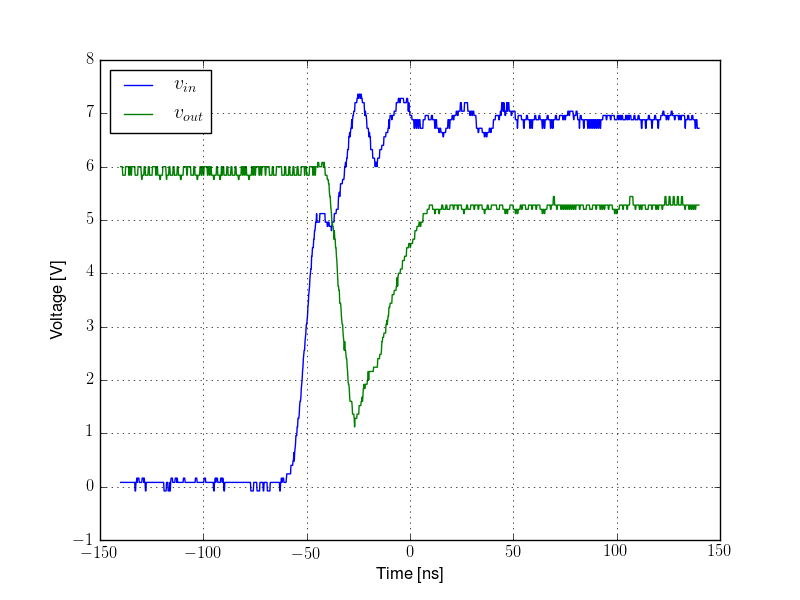
\includegraphics[width=.7\textwidth]{10/latency_plot.png}
\caption{The plot shows the delay caused by the propagation of the signal in 3 gates}\label{latency_plot}
\end{figure}
